
\section{Objetivo}

Que el alumno implemente y refuerce su comprensión del algoritmo A*.


\begin{auxcode}
 \caption{Pakuman}
 \centering
 \hurl{\auxprefix ia-pakuman-aestrella}
\end{auxcode}

\section{Introducci\'on}

El algoritmo A* es el algoritmo de búsqueda en el espacio de estados que tiene garantizado encontrar la solución de menor costo explorando la menor cantidad de estados en el espacio de búsqueda.  Para ello se beneficia de las propiedades del algoritmo de Dijkstra para encontrar la ruta mínima entre dos puntos de un grafo, aumentada con el uso de información del dominio a través de una función heurística, que estima la distancia faltante hasta la meta, permitiéndole así, explorar primero los caminos más prometedores.

Para que al ejecutar el algoritmo se cumplan estas características, la función heurística debe ser:
\begin{description}
 \item [Admisible] También le podemos decir \textbf{optimista}, nunca debe sobreestimar el costo hasta la meta.

 \item [Consistente] Ir directamente de un estado $A$ a un estado $B$ debe ser igual o menos costoso, que si hay una desviación pasando por $C$.  Esto se expresa en la desigualdad:
 \begin{align*}
  h(n) \leq c(n,a,n') + h (n')
 \end{align*}
 Donde el punto $A$ es el estado $n$ y $B$ es la meta.  Se debe cumplir entonces que la distancia estimada desde $n$ sea menor o igual que si se pasa por $n'$ al ejecutar la acción $a$.
\end{description}



\subsection{Navegación}

Un curso de Inteligencia Artificial no estaría completo sin haber implementado A*.  Una de las aplicaciones más populares de este algoritmo es el problema de navegación en videojuegos y robótica.  Comenzaremos siguiendo el ejemplo de Patrick \cite{Lester2003} en un mundo hecho de mosaicos.

En el ejemplo de Patrick, asumimos que tenemos un personaje que quiere ir desde un punto A hasta un punto B y que ambos puntos están separados por una pared. Este ejemplo se puede apreciar en la \fref{fig:AEstrellaIni}, donde el cuadrado verde es el punto A, el rojo es el punto B y el rectángulo gris, la pared mencionada anteriormente.  Curiosamente, este sencillo escenario no puede ser resuelto por ascenso de colinas, pero para A* es pan comido.

\begin{figure}
  \centering
  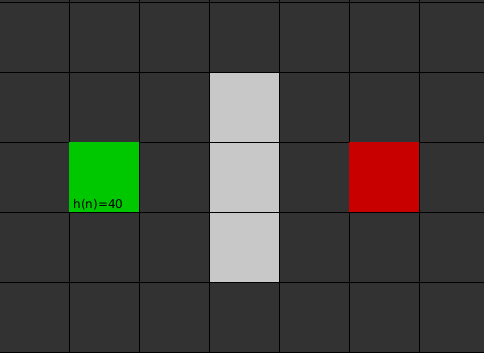
\includegraphics[width=0.4\textwidth]{aestrella/Barrera}
  \caption{Escenario construido con mosaicos discretos. El problema de búsqueda de caminos consiste en encontrar una ruta desde el cuadro verde al cuadro rojo.}
  \label{fig:AEstrellaIni}
\end{figure}

Si el mundo donde se encuentran nuestros personajes es continuo, como los ambientes donde se mueve un robot, el primer paso que debemos hacer es simplificar el área de búsqueda, dividiendo nuestro mundo en una rejilla de mosaicos.  En los videojuegos algunos mundos ya son así desde un prinicipio.  En el caso de robótica se puede proceder a crear rejillas de ocupación discretizando las coordenadas del plano y representando al mundo con mosaicos ocupados/libres, semejantes a los de los videojuegos.  Con esto, podremos representar el mundo con una matriz bidimensional. Cada posición en la matriz representará un mosaico del mundo, el cual será transitable o no transitable. Entonces, el objetivo del algoritmo A* es calcular a qué mosaico nos debemos mover en cada turno para lograr llegar al punto B. Una vez calculado esto, el personaje del juego se moverá del centro del mosaico donde se encuentra actualmente al centro del mosaico obtenido con A*.  Observa entonces que cada mosaico del mundo es un estado posible para nuestro personaje.


Ahora pensaremos en el mundo como un grafo, el puntos central de cada mosaico corresponde a un \textit{nodo}; de este modo los mosaicos podrían ser círculos, hexágonos o triángulos, no sólo cuadrados; cada mundo puede tener características diferentes y ser simplificado de distintas formas.  Cuando dos mosaicos son adyacentes y es posible desplazarse de uno hacia el otro, decimos que hay un arista conectándolos.  Así, el algoritmo que busca la ruta más corta entre el punto A y el punto B es un recorrido sobre un grafo.



\subsection{Iniciando la b\'usqueda}

Después de haber simplificado el área de búsqueda a un grafo con nodos y aristas, el siguiente paso es dirigir una búsqueda para encontrar el camino más corto.  Comenzamos por el punto A, luego consideramos los cuadros adyacentes (estados sucesores) para ver en qué dirección movernos y continuamos alejándonos hasta que encontremos nuestro destino.  Para ello utilizaremos dos estructuras a las cuales llamaremos \emph{lista abierta} y \emph{lista cerrada}.

\noindent Empezamos la búsqueda haciendo lo siguiente:

\begin{enumerate}
  \item Añadimos el punto inicial A a la \textbf{lista abierta}. Esta lista contiene los cuadrados que vamos a considerar para que formen parte del camino. Si, por azares del destino, el punto A es igual al punto B, terminamos nuestra ejecución con un plan vacío: el personaje no necesita hacer nada, ya está en su destino.
  
  \item Sacamos el cuadro inicial A de la lista abierta y lo añadimos a una \textbf{lista cerrada} de cuadrados que no necesitan ser considerados de nuevo.
  
  \item Nos fijamos en todos los cuadrados alcanzables o transitables adyacentes al punto de inicio, ignorando cuadrados no transitables (por contener muros, muebles, agua, precipicios, etc.). Se añaden a la lista abierta, marcando que el punto A es su \textbf{cuadrado padre}, pues estamos considerando llegar desde ahí. El cuadrado padre será muy importante para trazar nuestro camino al final de la búsqueda.  La estructura dentro de la cual guardaremos una referencia al cuadrado vecino y a su padre, y que ofreceremos a la lista abierta, se llama \textbf{nodo de búsqueda}.
\end{enumerate}

En este punto, se tendrá algo como la figura~\ref{fig:fig2P4}, en un momento explicaremos el significado de los números en las casillas. En este diagrama, el cuadrado verde es el \textbf{estado inicial} y ya ha sido añadido a la lista cerrada. Todos los cuadrados adyacentes están ahora en la lista abierta para ser considerados. Cada uno tiene un indicador que señala a su padre, que es el cuadro inicial.

\begin{figure}[h]
  \centering
  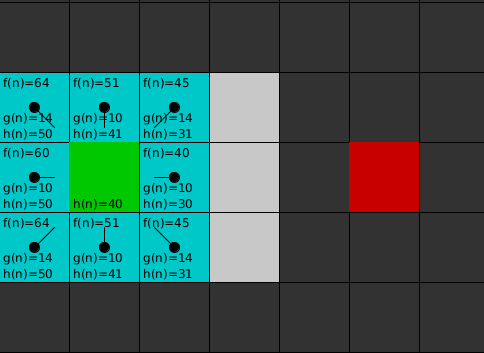
\includegraphics[width=0.6\textwidth]{aestrella/PrimerosVecinos.png}
  \caption{Mosaicos en la lista abierta con referencia a su padre.}
  \label{fig:fig2P4}
\end{figure}

Ahora necesitamos elegir a uno de los cuadrados de la lista abierta para explorar esa ruta. Elegimos aquel vecino que tenga costo estimado más bajo, es decir, aquel al que hemos llegado por la mejor ruta y promete estar más cerca de la meta, hasta donde sabemos, para ello calcularemos la función $f(n)$.

\subsection{Puntuando el camino}

Para determinar qué cuadrado exploraremos a continuación usaremos la siguiente ecuación:

\begin{center}
\(f(n) = g(n) + h(n)\)
\end{center}

donde:

\begin{itemize}
  \item \(g(n)\) es el costo del movimiento para ir desde el punto inicial A al cuadro \(n\) de la rejilla, siguiendo el mejor camino que se generó para llegar a $n$.

  \item \(h(n)\) es el costo estimado del movimiento para ir desde ese cuadro \(n\) hasta el destino final, el punto B. Si conociéramos ese costo exactamente no necesitaríamos buscar la mejor ruta, bastaría con movernos hacia el vecino con el valor más bajo, en lugar de ello sólo contaremos con una aproximación, a esta se le llama \textbf{heurística}.
\end{itemize}

Para generar el camino completo de A a B, tendremos que ir sacando a los nodos de la lista abierta con menor \(f(n)\) hasta llegar a la meta.  Sin embargo, calcular esta función requiere su truco, pues su valor puede cambiar conforme exploramos.  Veamos entonces cómo se hace ese cálculo.


\subsubsection{Heurística}

La primer función que podemos calcular es \(h(n)\), pues su valor no cambia una vez dado el ambiente.  Lo óptimo es calcularla la primera vez que el algoritmo ve al cuadrado \(n\), cuando crea el nodo búsqueda y lo inserta a la lista abierta.

Cuando se trata de problemas de desplazamiento, como es el caso aquí, una aproximación utilizada frecuentemente es la distancia Euclidiana (la ruta más corta, si no hubiera obstáculos, sería la línea recta), aunque tiene la desventaja de involucrar el cálculo de una raíz cuadrada. Por ello existen otras aproximaciones, que pueden ser más o menos adecuadas, dependiendo del ambiente.

Además de la distancia Euclidiana, otra técnica para aproximar distancias es el método Manhattan, donde se calcula el número total de cuadros movidos horizontalmente y verticalmente para alcanzar el cuadrado destino desde el cuadro actual, sin hacer uso de movimientos diagonales e ignorando cualquier obstáculo. Se llama método Manhattan porque está inspirado en el distrito que lleva ese nombre, donde las calles están diseñadas en forma de rejilla y para ir desde un lugar a otro no es posible tomar atajos atravesando una manzana en diagonal.  Observa que esta estimación es mejor si el agente no puede moverse en diagonal, pues de este modo nunca sobreestimará qué tan lejos está la meta.

En esta práctica asignaremos un costo de 10 por cada movimiento vertical u horizontal a través de un cuadrado y un costo de 14 para un movimiento diagonal (una aproximación razonable de \(\sqrt{2}\times10\)), pues usar números enteros es mucho más rápido para la computadora y la diferencia en tiempo puede ser significativa si el algoritmo se ejecutará muchas veces sobre muchos nodos.

Las puntuaciones \(h(n)\) se calcularán estimando la distancia Manhattan desde $n$ hasta el cuadrado objetivo (en rojo), moviéndose solo horizontal y verticalmente e \textbf{ignorando el muro} que está en el camino. Usando este método, en la \fref{fig:fig2P4} el cuadro a la derecha del inicial, está a 3 cuadros del cuadrado rojo lo que da una puntuación \(h(n)\) de 30. Los cuadrados arriba y abajo del incial están a sólo 4 cuadros de distancia (tomando sólo movimientos en dirección horizontal y vertical), dando una puntuación \(h(n)\) de 40.


\subsubsection{Costo parcial}

La siguiente función a estimar es \(g(n)\), el costo del movimiento para ir desde el punto de inicio al cuadro \(n\), usando el camino generado para llegar ahí.  Observa que por lo mismo, solamente se puede calcular conforme se van eligiendo los nodos durante la búsqueda.

Una vez calculado el costo \(g(n)\), el costo \(g(n')\) para su vecino $n'$, al que estamos llegando, es \(g(n)\) más 10 o 14 dependiendo de si el movimiento para llegar a él es ortogonal o se realiza en diagonal desde su cuadro padre.

En la \fref{fig:fig2P4} se pueden ver estos cálculos.  En el cuadrado a la derecha del inicial \(g(n)=10\). Esto es debido a que está solo a un cuadro del cuadrado inicial en dirección horizontal. Los cuadrados inmediatamente encima, abajo y a la izquierda del cuadrado inicial tienen todos el mismo valor \(g(n)\) de 10. Los cuadros diagonales tienen un valor \(g(n)\) de 14.  \(f(n)\) se calcula sumando \(g(n)\) y \(h(n)\).


\subsection{Continuando la b\'usqueda}

Para continuar la búsqueda, se elige al nodo con la puntuación \(f(n)\) más baja de todos aquellos que estén en la lista abierta. Para que esta operación se realize lo más eficientemente posible, la lista abierta se debe implementar con una cola de prioridades. Después hacemos lo siguiente con el cuadro seleccionado:

\begin{enumerate}
  \item Lo sacamos de la lista abierta y lo añadimos a la lista cerrada.  

  \item Comprobamos todos los cuadrados adyacentes:
  
  \begin{enumerate}
   \item Ignorando aquellos que estén en la lista cerrada o que sean intransitables o a los que no se puede pasar: terrenos con muros, agua o cualquier terreno prohibido.
   
   \item Añadimos los cuadros a la lista abierta si no están ya en esa lista. Hacemos que el cuadro seleccionado sea el \textbf{padre} de los cuadros nuevos.
   
   \item Si el cuadro adyacente ya está en la lista abierta, comprobamos si el camino nuevo a ese cuadro es mejor que el que tenía, es decir, si el valor de \(g(n)\) con este padre es menor que el que se había estimado con su padre anterior. Si no es así, no haremos nada. Por otro lado, si el costo \(g(n)\) del nuevo camino es más bajo, cambiamos el padre del cuadro adyacente al cuadro seleccionado (en el diagrama superior, cambia la dirección del puntero para que señale al cuadro seleccionado). Finalmente, recalculamos \(f(n)\) y \(g(n)\) para ese cuadrado.
  \end{enumerate}
\end{enumerate}


\begin{figure}[h!]
  \centering
  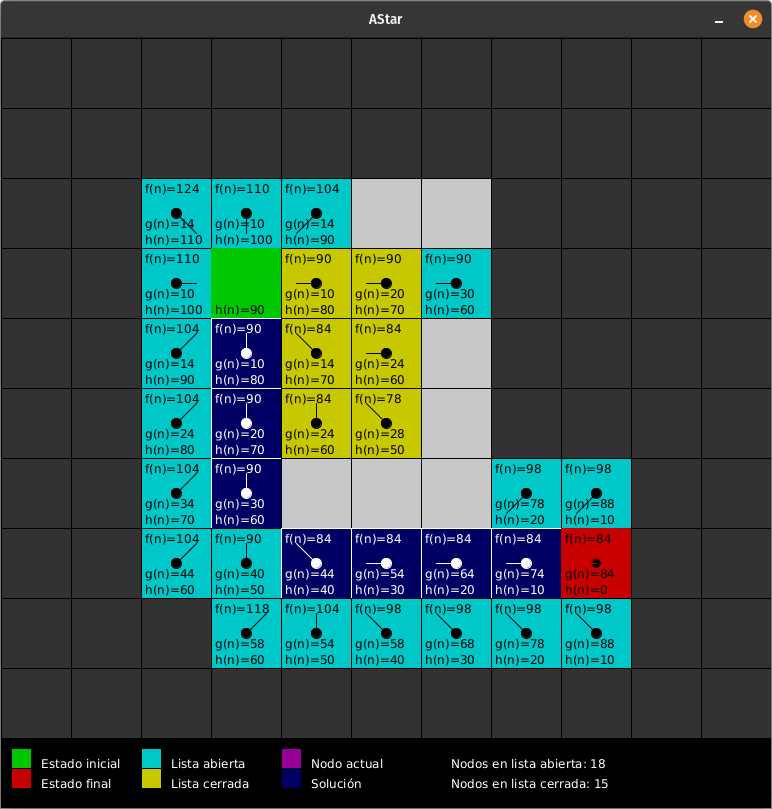
\includegraphics[width=0.95\textwidth]{aestrella/AEstrellaNoAdmisible.png}
  \caption{Ejecución completa del algoritmo con distancia Manhattan. A* encuentra una ruta, pero no es la óptima.}
  \label{fig:NoAdmisible}
\end{figure}

\begin{figure}[h!]
  \centering
  \includegraphics[width=0.95\textwidth]{aestrella/screen5.png}
  \caption{Ejecución completa del algoritmo con distancia Euclidiana.  A* encuentra la ruta óptima.}
  \label{fig:fig4P4}
\end{figure}


A continuación se muestran dos versiones de la ejecución completa del algoritmo para un escenario ligeramente más complejo.  En la primer versión usamos distancia Manhattan.  La \fref{fig:NoAdmisible} muestra el contenido final de las estructuras auxiliares, las listas cerrada y abierta y los valores calculados de $h$, $g$ y $f$.  Observa que, para este mapa donde se permiten movimientos en diagonal, esta heurística no es \textbf{admisible}, pues la ruta más corta puede utilizar diagonales y, entonces, estar más cerca de lo que estima.  La consecuencia es que A* no siempre encuentra la ruta óptima en estas condiciones.  La \fref{fig:fig4P4} muestra lo que sucede cuando se usa la distancia Euclidiana, que sí es una heurística admisible.


\section{Desarrollo e implementaci\'on}

Para esta práctica, considérate un miembro nuevo en un compañía de programación de videojuegos.  El resto del equipo ha estado trabajando en un \textit{remake} de Pacman con \code{JavaFX} y a ti te han asignado la siguiente tarea: programar al más férreo perseguidor de Pacman, el fantasma rojo \textbf{\textit{Sombra}}, mejor conocido como Blinky. Para ello, has decidido utilizar el mejor algoritmo para mundos finitos deterministas: A*.

Para realizar esta tarea se te entrega el código con el escenario listo para jugar y la documentación que han elaborado tus colegas.  El código aún no está terminado, pero ya incluye como muestra el primer nivel del juego y está listo para añadirle archivos de configuración con cualquier otro nivel.  Igualmente el código para controlar a Pacman usando las flechas del teclado ya funciona.  El único detalle es que Sombra aún no persigue a Pacman, se mueve siempre en una dirección fija que, lo notarás de inmediato, no lo lleva muy lejos.

El programa está compuesto por varios paquetes y clases pero como está diseñado con orientación a objetos, sólo necesitas entender algunas clases para agregar el algoritmo que necesita Sombra.  El diagrama UML de la \fref{fig:umlestrella} te muestra los paquetes, clases, atributos y métodos que son relevantes para tu tarea.

\begin{sidewaysfigure}
  \centering
  \includegraphics[width=\textwidth]{aestrella/UMLSombra.png}
  \caption{UML con las clases relevantes para programar el algoritmo de navegación para Sombra.  Las clases con métodos a implementar se muestran en rosa.}
  \label{fig:umlestrella}
\end{sidewaysfigure}

\subsection{Implementaci\'on}

Tu trabajo consiste en implementar la función:

\code{LinkedList<Movimiento> resuelveAlgoritmo(Estado estadoInicial, Estado estadoFinal)}

\noindent de la clase \code{pacman.personajes.navegacion.AEstrella}.
La variable \code{estadoInicial} contiene información con las coordenadas de la casilla inicial, mientras que \code{estadoFinal} indica a qué casilla se quiere ir.  El trabajo de esta función es devolver la secuencia de acciones que se deben realizar (movimientos) hasta llegar a la casilla final.

Para que ubiques mejor cómo será usada esta función te informan que, de momento, el estadoInicial corresponde a la posición actual de Sombra y estadoFinal es la posición de Pacman.  Sombra manda llamar esta función en cada tick del reloj con las nuevas posiciones suya y de Pacman.  De hecho, lo único que se utiliza es el primer movimiento de la trayectoria... pero no te confíes, las cosas pueden cambiar, otras optimizaciones podrían ser introducidas y por lo tanto debes calcular la lista completa de movimientos.  Aunque estos detalles son irrelevantes para tu código, saber cómo será usado te ayudará a visualizar lo que necesitas hacer.  Sin embargo, observa que por ser general, esta función podría llegar a utilizarse no sólo para mover a Sombra sino que, en algún momento, otro fantasma con otro comportamiento también podría aprovecharla.  Por ejemplo, el encargado de las emboscadas \textbf{\textit{Pinky}} podría usar A* para llegar a la esquina más cercana a Pacman enviando como parámetros sus coordenadas y las de dicha esquina.  Por lo tanto, no debes usar información de más o de menos confiándote en el estado actual de la aplicación, ni afectar el resto del juego con intervenciones innecesarias para que tu código sea reutilizable con facilidad.

Para ayudarte a realizar esta tarea el paquete te ofrece las herramientas siguientes:

\begin{enumerate}
 \item La clase \code{Estado} pertenece al subpaquete \code{navegación}.  Es una especie de envoltura con una referencia a un \code{Pasillo} por donde puede pasar el fantasma.  Un objeto de este tipo puede almacenar la información de ejecución relevante para el algoritmo A* como es el valor de la función \(h(n)\).  De este modo te brinda acceso al estado en el mundo (el laberinto donde se encuentran nuestros personajes) y te brinda un espacio para no afectar al mundo con información que sólo concierne al algoritmo de navegación de un fantasma.
 
 \item La superclase \code{Algoritmo} se encarga de inicializar, tras la creación del laberinto, un arreglo de objetos tipo \code{Estado}.  De este modo cuentas ya con un objeto estado por cada pasillo en el laberinto, en el mismo renglón y columna que el pasillo en el mundo.  Ojo, los valores de la heurística $h(n)$ cambian cada vez que cambia el lugar al que quiere moverse el fantasma, así que recuerda recalcular tantos valores como sean necesarios cada vez que ejecutes el algoritmo con metas distintas.
 
 \item La clase \code{NodoBusqueda} contiene la información del grafo de búsqueda que va generando A* conforme explora los estados.  Por eso su primer atributo es una referencia al estado que está explorando.  También aquí se almacena el valor de $g(n)$, pues este valor depende de la ruta que se siga para llegar al estado $n$ desde el estado inicial; por ello mismo incluye la referencia al nodo padre y la acción que se realizó para llegar al estado que contiene.  Recuerda que, en general, varios nodos de búsqueda podrían apuntar al mismo estado.  Como en esta práctica se realizará una búsqueda en grafo no será el caso.
 
 \item La clase \code{Pasillo} ya representa, de hecho, la gráfica de estados por donde puede transitar un personaje, pues cada pasillo contiene referencias a sus pasillos vecinos.  Puedes acceder a ellos mediante el método \code{obtenVecino(Movimiento mov)}.  Te servirá para generar los estados sucesores de cada estado.
\end{enumerate}

Los métodos que deberás implementar son los siguientes:

\begin{enumerate}
 \item En la clase \code{Estado} la función:
 \begin{enumerate}
  \item \code{calculaHeuristica(Estado meta)}
 \end{enumerate}

 \item En la clase \code{NodoBusqueda}:
 \begin{enumerate}
  \item \code{LinkedList<NodoBusqueda> getSucesores()}
 \end{enumerate}


 \item En la clase \code{AEstrella}:
 \begin{enumerate}
  \item \code{LinkedList<Movimiento> resuelveAlgoritmo(Estado estadoInicial, Estado estadoFinal)}
 \end{enumerate}
 se te sugiere la implementación de dos métodos auxiliares:
 \begin{enumerate}
  \item \code{inicializa(Estado estadoInicial, Estado estadoFinal)}
  \item \code{void expandeNodoSiguiente()}
 \end{enumerate}
 Como son métodos privados, tienes la libertad de utilizarlos o modificarlos a tu gusto.  Se te provee con \code{pintaTrayectoria(Color color)} para ayudarte a depurar tu código.

\end{enumerate}

\section{Requisitos y resultados}

Los requisitos para tu trabajo son los siguientes:

\begin{enumerate}
 \item Para implementar el algoritmo puedes agregar atributos sólo si realmente necesitas recordar los valores de esas variables entre distintas llamadas a los métodos de la clase, únicamente en las clases marcadas con rosa.
 
 \item Es estas clases también puedes agregar métodos auxiliares si lo consideras necesario. De hacerlo, no olvides documentar cual es su función.
 
 \item No debes agregar ni atributos ni funciones a ninguna otra clase, ya tienes toda la información que necesitas; piensa que el resto del programa está siendo desarrollado por otros compañeros de la empresa y no tienes permiso de tocar sus componentes.
\end{enumerate}

Cuando termines tu implementación podrás ver a Sombra persiguiendo a Pacman por la ruta óptima; la única forma de alejarlo un poco será transportándote por los pasillos que sacan a Pacman por un lado de la pantalla y lo regresan por el otro.  Si gustas, borrar e iluminar la ruta que sigue Sombra a cada paso es muy fácil ya teniendo la trayectoria completa.

\begin{figure}
  \centering
  \includegraphics[width=0.4\textwidth]{aestrella/screen6.png}
  \caption{Sombra persiguiendo a Pacman por la ruta óptima.}
  \label{fig:fig1P4}
\end{figure}
